	\section{K-means Clustering}

	\resetquestioncounter{}

	\begin{qanda}
		\begin{question}
What is K-means clustering?
		\end{question}

		\begin{answer}
K-means is a centroid-based algorithm, or a distance-based algorithm, where we calculate the distances to assign a point to a cluster. In K-Means, each cluster is associated with a centroid.
		\end{answer}
	\end{qanda}

	\begin{qanda}
	\begin{question}
What are some good things about K-means clustering?
	\end{question}

	\begin{answer}
Some benefits include:
	\begin{bulletedlist}
		\item It is very smooth in terms of interpretation and resolution.
		\item For a large number of variables present in the data set, K-means operates quicker than hierarchical clustering.
		\item While redetermining the cluster center, an instance can modify the cluster.
		\item K-means reforms compact clusters.
		\item It can work on unlabeled numerical data.
	\end{bulletedlist}
	\end{answer}
	\end{qanda}

	\begin{qanda}
		\begin{question}
What are the limitations of K-means clustering?
		\end{question}

		\begin{answer}
Some limitations include:
	\begin{bulletedlist}
		\item Sometimes, it is quite tough to figure out the appropriate number of clusters, or the value of k.
		\item The output is highly influenced by the original input, for example, the number of clusters.
		\item It gets affected by the presence of outliers in the data set.
		\item In some cases, clusters show complex spatial views, then executing clustering is not a good choice.
	\end{bulletedlist}
		\end{answer}
	\end{qanda}

	\begin{qanda}
		\begin{question}
Is there any metric to compare clustering results?
		\end{question}

		\begin{answer}
You can compare clustering results by checking silhouette scores and by doing cluster profiling. Besides this, you should also validate the clustering results by consulting with a domain expert to see if the cluster profiles make sense or not.
		\end{answer}
	\end{qanda}


	\begin{qanda}
		\begin{question}
For K-means if there is a y-dependent variable, do we remove it before trying to group customers?
		\end{question}

		\begin{answer}
Yes, if you have a dependent variable in your dataset, you should remove that before applying clustering algorithms to your dataset.
		\end{answer}
	\end{qanda}

	\begin{qanda}
		\begin{question}
How do we select the optimal number of clusters from the Elbow curve?
		\end{question}

		\begin{answer}
Choosing the optimal number of clusters is a fairly subjective matter, and the best method to identify the optimum number of clusters is to use a combination of metrics and domain expertise. The Elbow curve is one of the most common ways of finding the right number of clusters for K-Means clustering if we don't have domain expertise. The elbow curve is plotted between the number of clusters on the X-axis and WCSS (within the cluster sum of squares) on the Y-axis.

The elbow method uses the WCSS to choose an ideal value of k based on the distance between the data points and their assigned clusters. WCSS is the sum of the squared distance between each point and the centroid in a cluster. We would choose a value of k where the WCSS begins to flatten out, and we see an inflection point.

The graph above shows that k = 4 is an appropriate number of clusters to choose from, with an obvious elbow at that number. At K=4, the graph shows a significant fall in WCSS. As a result, 4 is the best K-value.
		\end{answer}
	\end{qanda}

	\begin{figure}[h]
		\centering
		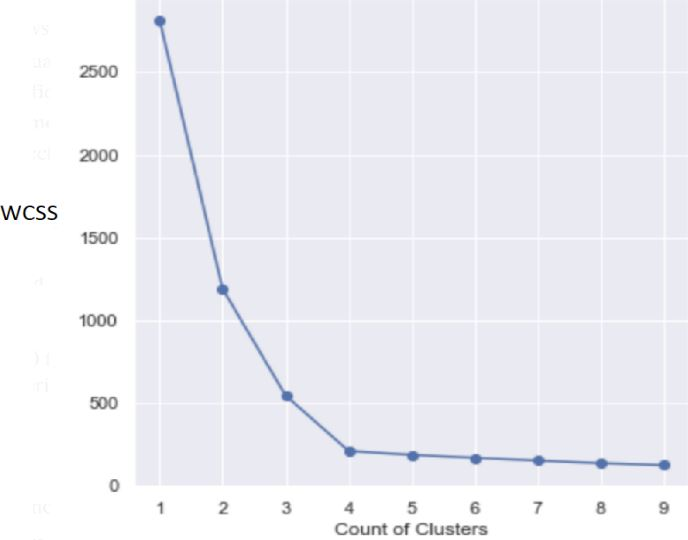
\includegraphics[height=2.5in]{kmeansclustering}
		\caption[K-means clustering]{K-means clustering.}
		\label{fig:kmeansclustering}
	\end{figure}


	\begin{bulletedlist}
		\item K-Means is probably the most used clustering technique.
		\item Aims to partition the n observations into k clusters so as to minimize the within-cluster sum of squares (i.e. variance).
		\item Computationally less expensive compared to hierarchical techniques.
		\item Have to pre-define K, the no of clusters.
		\item Requires data to be scaled first.  The most popular method of scaling is to use z-scores.
	\end{bulletedlist}


	\begin{table}
        \centering
        \caption[Strengths and weaknesses of k-means clustering]{Strengths and weaknesses of k-means clustering.}
        \label{tab:}
		\begin{tabular}{|p{0.5\textwidth-2\tabcolsep}|p{0.5\textwidth-2\tabcolsep}|} \hline
			\tablecolumnheadervlinesone{Strengths} & \tablecolumnheadervlinestwo{Weakness} \\ \hline
			Use simple principles without the need for any complex statistical terms. &
			How to choose K? \\ \hline
			Once clusters and their associated centroids are identified, it is easy to assign new objects (for example, new customers) to a cluster based on the object's distance from the closest centroid. &
			The k-means algorithm is sensitive to the starting positions of the initial centroid. Thus, it is important to rerun the k-means analysis several times (with different random starting points) for a particular value of k to ensure the cluster results provide the overall minimum within-cluster-sum of squared errors (WSS). \\ \hline
			Because the method is unsupervised, using k-means helps to eliminate subjectivity from the analysis. &
			Susceptible to curse of dimensionality. \\ \hline
		\end{tabular}
	\end{table}

	\subsection{Lloyd's algorithm}

	\begin{numberedlist}
		\item Assume K centroids.
		\item Compute Squared Euclidean distance of each objects with these K centroids. Assign each to the closest centroid forming clusters.
		\item Compute the new centroid (mean) of each cluster based on the objects assigned to each clusters.
		\item Repeat 2 and 3 till convergence: usually defined as the point at which there is no movement of objects between clusters.
	\end{numberedlist}

	\begin{bulletedlist}
		\item Usually subjective, based on striking a good balance between compression and accuracy.
		\item The ``elbow'' method is commonly used.
	\end{bulletedlist}

	\begin{figure}[h]
		\centering
		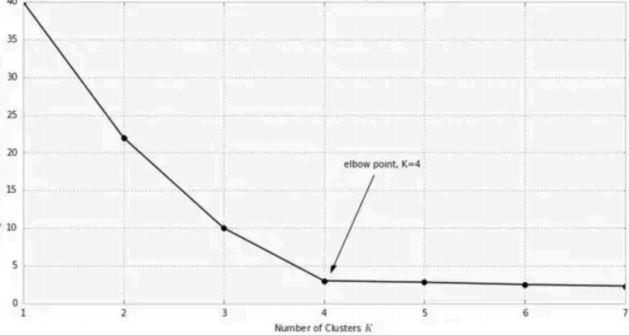
\includegraphics[height=2.5in]{elbowmethod}
		\caption[Elbow method of finding the optimum number of clusters]{Elbow method of finding the optimum number of clusters.}
		\label{fig:elbowmethod}
	\end{figure}

	\subsection{Silhouette Coefficient for K-Means}
	\begin{numberedlist}
		\item Calculate average distance of a point to all other points in the group ($a_i$).
			\begin{numberedlist}
				\item Select a point.
				\item Compute the sum of the distances from that point to all others in the cluster.
				\item Divide by the number of points in the cluster minus 1 (number of distances calculated).
			\end{numberedlist}
		\item Calculate the average distance from that same point to all the points in another group.
		\item Take the minimum of the average distances to all other clusters ($b_i$).
		\item Calculate
	\end{numberedlist}

	\begin{equation}
		S_i = \left\{ \begin{array}{r@{\quad : \quad}ll}
									1-\frac{a_i}{b_i}    &   a_i < b_i  & \text{distance of point $i$ to another cluster}    \\
                                            0            &   a_i = b_i  & \text{two clusters are the same}    \\
                                    \frac{a_i}{b_i}-1    &   a_i > b_i  & \text{point $i$ is closer to another cluster than its own}    \\
                      \end{array}\right.
	\end{equation}

The silhouette measurement is in the range of [-1, 1] (inclusive end points).

	\subsection{Visual Analysis of Clustering}
	\begin{bulletedlist}
		\item Visual analysis of the attributes selected for the clustering may given an idea of the range of values that K should be evaluated in.
		\item Identifying the attributes on which clusters are clearly demarcated and using them in incremental order to build the multi-dimensional clusters likely to give much better clusters than using all the attributes at one go.
		\item A kernel density estimate plot can be used to see clusters in individual features (columns).
	\end{bulletedlist}

	\begin{figure}[h]
		\centering
		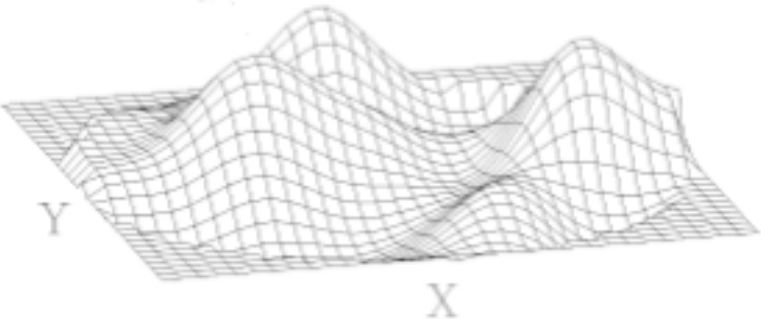
\includegraphics[height=2.5in]{clusteringvisualization}
		\caption[Clustering visualization]{Clustering visualization.}
		\label{fig:clusteringvisualization}
	\end{figure}

	\subsection{Dynamic Clustering}
	\begin{bulletedlist}
		\item Clustering on correct attributes is the key to good clustering results.
		\item We can also consider those attributes who's value changes with time. For e.g. age, income category, years of work experience etc.
		\item We can use sequential k means clustering over time to track individual clusters (how they change in size, shape and position
		\item We can also understand how individual data points move across clusters, form new clusters etc.
		\item Analyzing the changes in the clusters over time using metrics such as
		\item Cluster size, new entries and exits one can analyze the impact of strategies designed based on earlier clustering analysis
	\end{bulletedlist}
